\section{The error estimate}

Solving PDEs numerically will result in errors because derivatives are approximated by finite differences and the PDE is required to be fulfilled only on the mesh points. 
For the schemes used in this thesis the error, $\epsilon$ will follow equation \eqref{analysis:error}

\begin{equation}\label{analysis:error}
 \epsilon = C_x\Delta x^2 + C_t\Delta t
\end{equation}

\noindent where the coefficients $C_x$ and $C_t$ are unknown. 
Notice that there is one term arising from the time derivative and one from the spatial derivative and that they are of different order. 

The error is measured by comparing the result from a numerical simulation to an exact solution, $u_e$ and taking the norm of the difference. 
Specifically $\epsilon$ is measured by the L2 norm which is defined in equation \eqref{analysis:def_epsilon}
% \label{analysis:def_epsilon}
\begin{align}
 \epsilon(t^n) &= ||u(t^n)-u_e(t^n)||_2 \nonumber \\
 &= \iint\sqrt{\left(u(t^n,x,y)-u_e(t^n,x,y)\right)^2}\,dx\,dy \nonumber \\
 &\approx \sqrt{\Delta x\Delta y\sum\limits_{i=0}^n\sum\limits_{i=0}^n \left(u(t^n,x_i,y_j)-u_e(t^n,x_i,y_j)\right)^2}\label{analysis:def_epsilon}
 \end{align}
 
\noindent $\epsilon$ is time dependent because it allows for investigation of the evolution of the error over the course of a simulation.
Some of the error tests will require a single number as an error measure. 
In these cases the norm of $\epsilon(t)$, defined in eq. \eqref{analysis:convergence_test_error} is used.
\begin{equation}\label{analysis:convergence_test_error}
 \epsilon = \sqrt{\Delta t\sum\limits_{n=0}^T\epsilon(t^n)^2}
\end{equation}

\section{Verification techniques}

This thesis will focus on three verification techniques which are described below. 
The aim for all of these techniques is to make sure that the implementation is correct by comparing simulations results known to be correct. 
% The aim for all of these techniques is to make sure that the error term follows equation \eqref{analysis:error}. 
Since an incorrect implementation of the spatial derivative will cause the solution to be unstable which is easily noticed through visual inspection, the tests will focus on verifying the time derivative. 
Isolating the contribution to $\epsilon(t)$ from the time derivative will be necessary and is ensured by setting $\Delta t \gg\Delta x^2$. 
A time step of this size violates the stability criterion for the FE scheme, and so some of the tests are slightly inaccurate for this scheme. \\

The verification techniques are

\begin{itemize}
 \item Manufactured solutions\\
 By modifying the source term almost any solution can be chosen, hence the name ``manufactured solutions''. 
%  By choosing an adequate initial condition the exact solution to the diffusion equation can be found with relative ease. 
 The chosen solution is
 \begin{equation}\label{manufactured_solution}
  u(x,y,t) = e^{-\pi^2t}\cos(\pi x)\cos(\pi y) +1
 \end{equation}
 which requires no source term. 
  The point of these tests is to verify that $\epsilon \sim \Delta t$ and the tests can be done for a time step which fulfills the stability criterion.
  \item Convergence tests \\
  In the general case the error term is proportional to the time step to some power $r$ when the error from the time derivative is dominant.
\begin{equation}
 \epsilon \simeq C_t\Delta t^r
\end{equation}
By comparing the error from two simulations with different time steps the exponent $r$, called the convergence rate, can be found
\begin{align*}
 \epsilon_1 &\simeq C_t\Delta t_1^r\\
  \epsilon_2 &\simeq C_t\Delta t_2^r
  \end{align*}
  the two expressions are divided
  \begin{align*}
   \frac{\epsilon_1}{\epsilon_2} &\simeq \frac{C_t\Delta t_1^r}{C_t\Delta t_2^r}\\
   \log\left(\frac{\epsilon_1}{\epsilon_2}\right) &\simeq r\log\left(\frac{\Delta t_1}{\Delta t_2}\right)\\
   r&\simeq \frac{\log\left(\epsilon_1/\epsilon_2\right)}{\log\left(\Delta t_1/\Delta t_2\right)}
\end{align*}
The FE and BE schemes have errors proportional to $\Delta t$ so the tests are expected to measure $r=1$. 
For these tests it is better if the time step is larger than the stability criterion for the FE scheme.
  \item Exact numerical solutions \\
  The numerical schemes are actually reformulations of the PDE we are trying to solve as difference equations which have their own exact solutions. 
  These will be called the numerical exact solutions, and they are slightly different from the exact solutions to the PDE. 
  The reason for finding the numerical exact solutions is that the scheme theoretically will represent this solution with no error. 
  In practice there will always be round off errors and other factors, but an error term close to machine precision is expected.
\end{itemize}

\section{Testing the PDE solver}


\subsection{Verification by manufactured solutions}

Equation \eqref{manufactured_solution} solves the diffusion equation, so using $u(x,y,t=0)$ as the initial condition for a simulation will give us both the numerical solution and the exact solution. 
An important property of the discretization scheme is that the difference between these solutions is of the same order as the time step.
\begin{equation*}
 \epsilon(t) \sim \mathcal{O}(\Delta t)
\end{equation*}
\noindent For the FE scheme a single discretization parameter will be introduced by having a constant relation between the spatial resolution and the time step 
\begin{equation*}
 \frac{\Delta t}{\Delta x^2} = k
\end{equation*}
$\epsilon(t)$ can now be rewritten by setting $\Delta t = h$
\begin{align*}
 \epsilon(t) &= C_t h + C_x\frac{h}{k} \\
 &= (C_t +C_x/k)h = C_k h
\end{align*}

Figures \ref{analysis:errorplots:FE} and \ref{analysis:errorplots:BE} show that for both the FE and BE scheme in both 1D and 2D the error is of the expected magnitude. 
Another interesting property of the error plots is that the error tends to zero after a large number of time steps. 
By inserting the limit $t\to\infty$ in \eqref{manufactured_solution} we observe that the error is expected to tend to zero because the limit value of one can be exactly recreated by both schemes.
\begin{align*}
 \lim_{t\to\infty} e^{-\pi^2t}\cos(\pi x)\cos(\pi y) +1 = 1
\end{align*}

\begin{figure}[H]
% Error plots for FE in 1D (a) and 2D (b)
 \centering
 \begin{subfigure}{0.49\textwidth}
  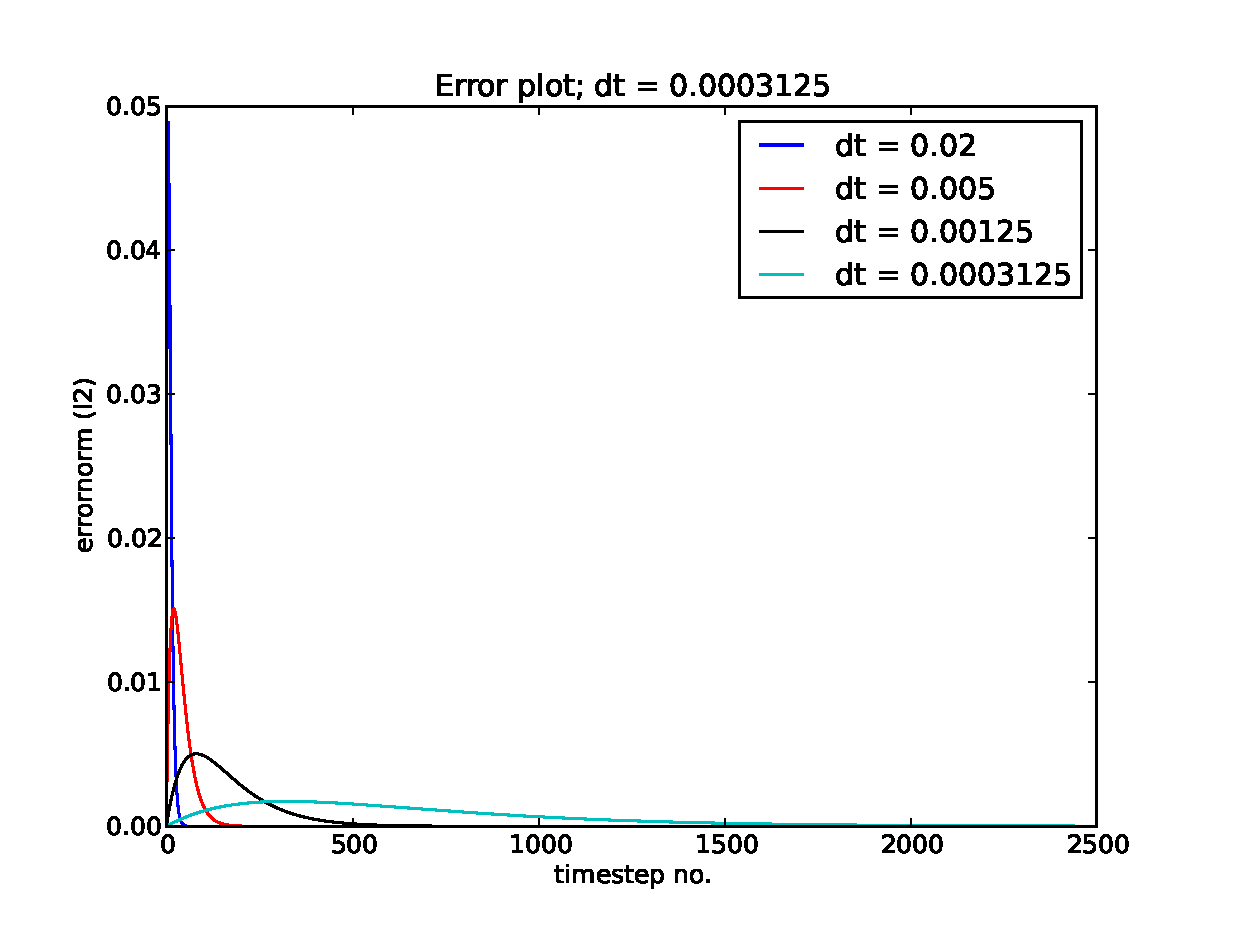
\includegraphics[width=\textwidth]{../results/experiment_18042014_1014_convergencetest_FE1D/results/errorplot.eps}
  \caption{}
 \end{subfigure}
 \begin{subfigure}{0.49\textwidth}
  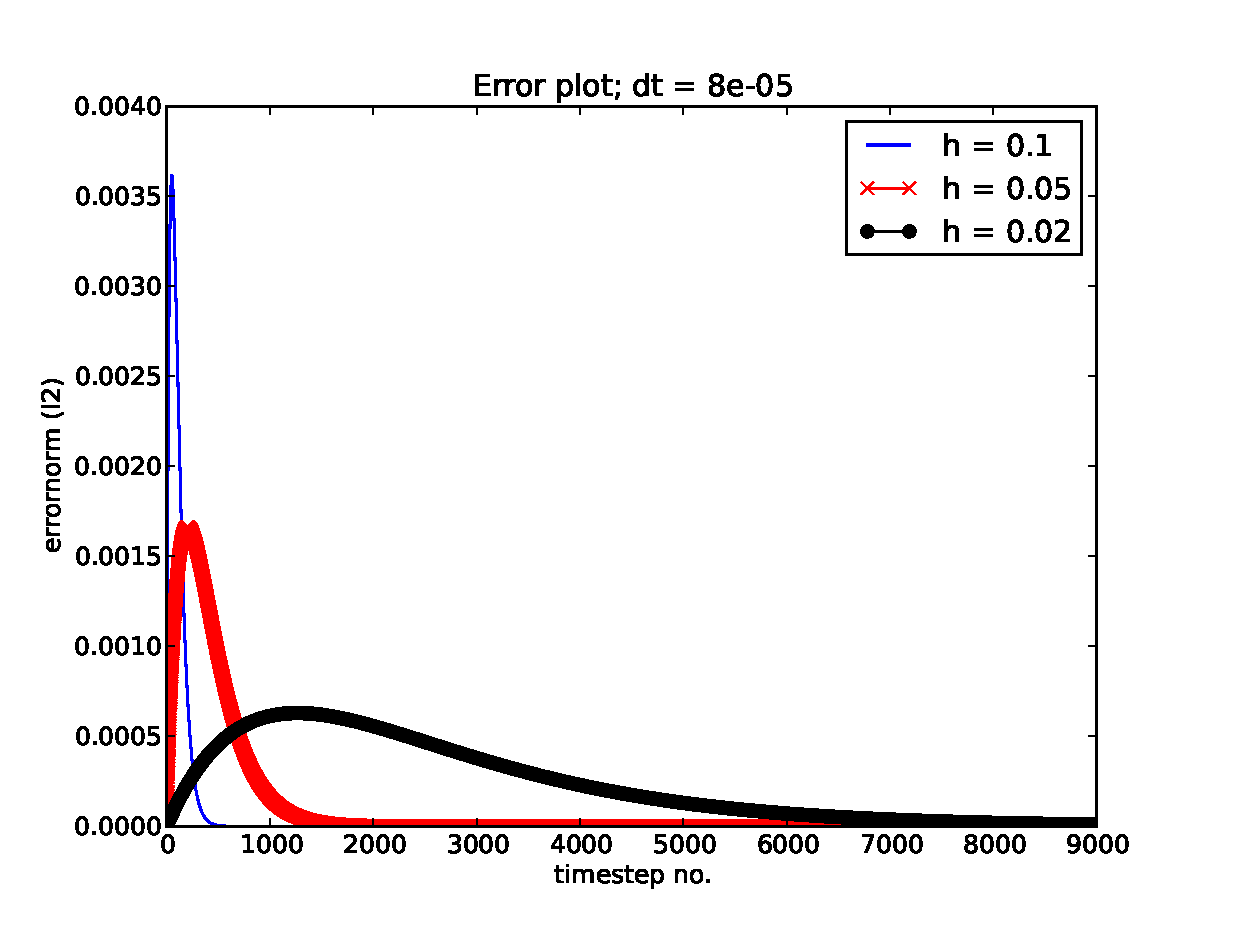
\includegraphics[width=\textwidth]{../results/experiment_14052014_0754_errorplot_FE2D/results/errorplot.eps}
  \caption{}
 \end{subfigure}
 \caption[Error plots FE]{Error plot for the FE scheme in 1D (a) and 2D (b). Note that there is now only one discretization parameter called $h$.}
 \label{analysis:errorplots:FE}
\end{figure}


\begin{figure}[H]
% Error plots for BE in 1D (a) and 2D (b)
\centering
 \begin{subfigure}{0.49\textwidth}
  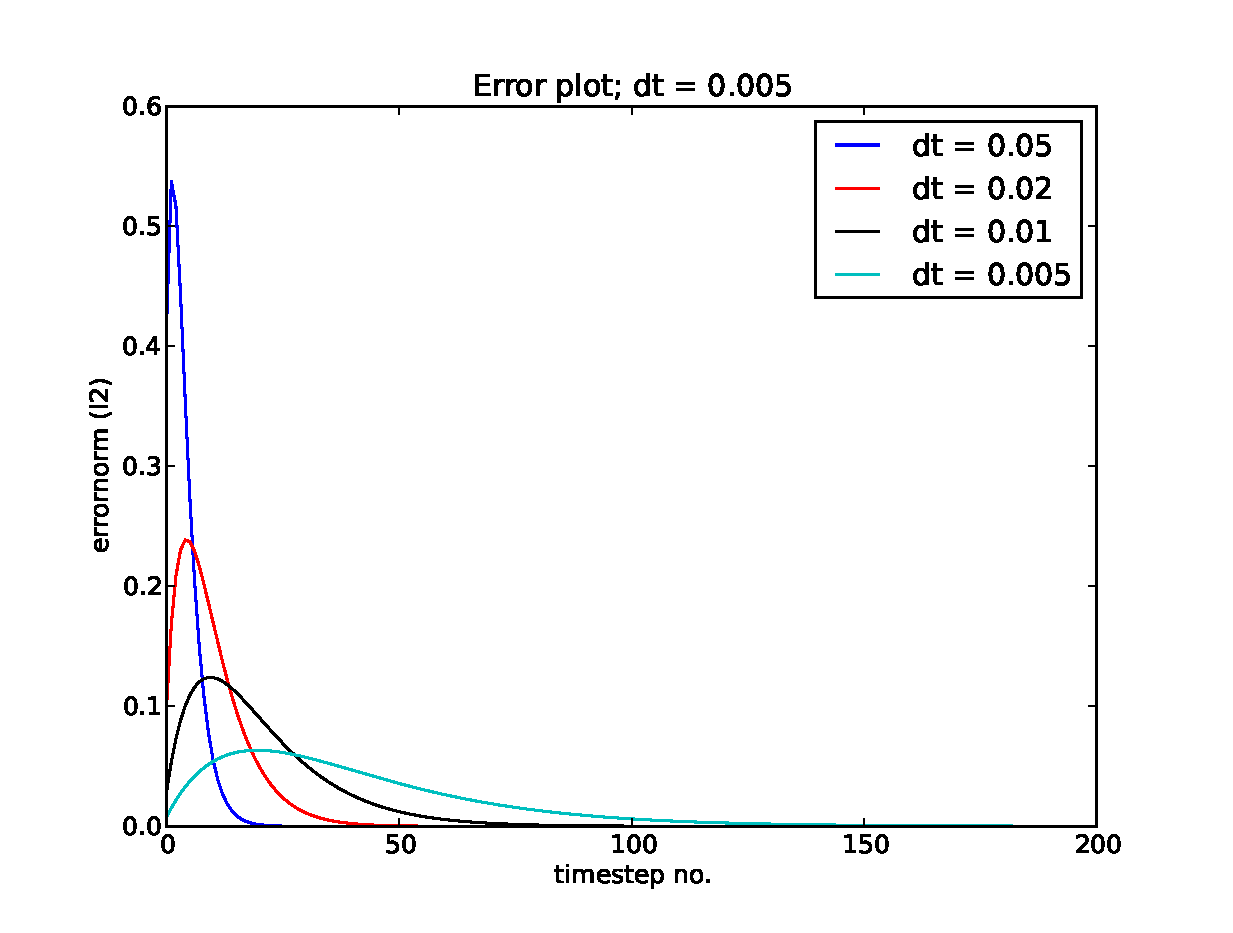
\includegraphics[width=\textwidth]{../results/experiment_14052014_0744_errorplot_BE1D/results/errorplot.eps}
  \caption{}
 \end{subfigure}
 \begin{subfigure}{0.49\textwidth}
  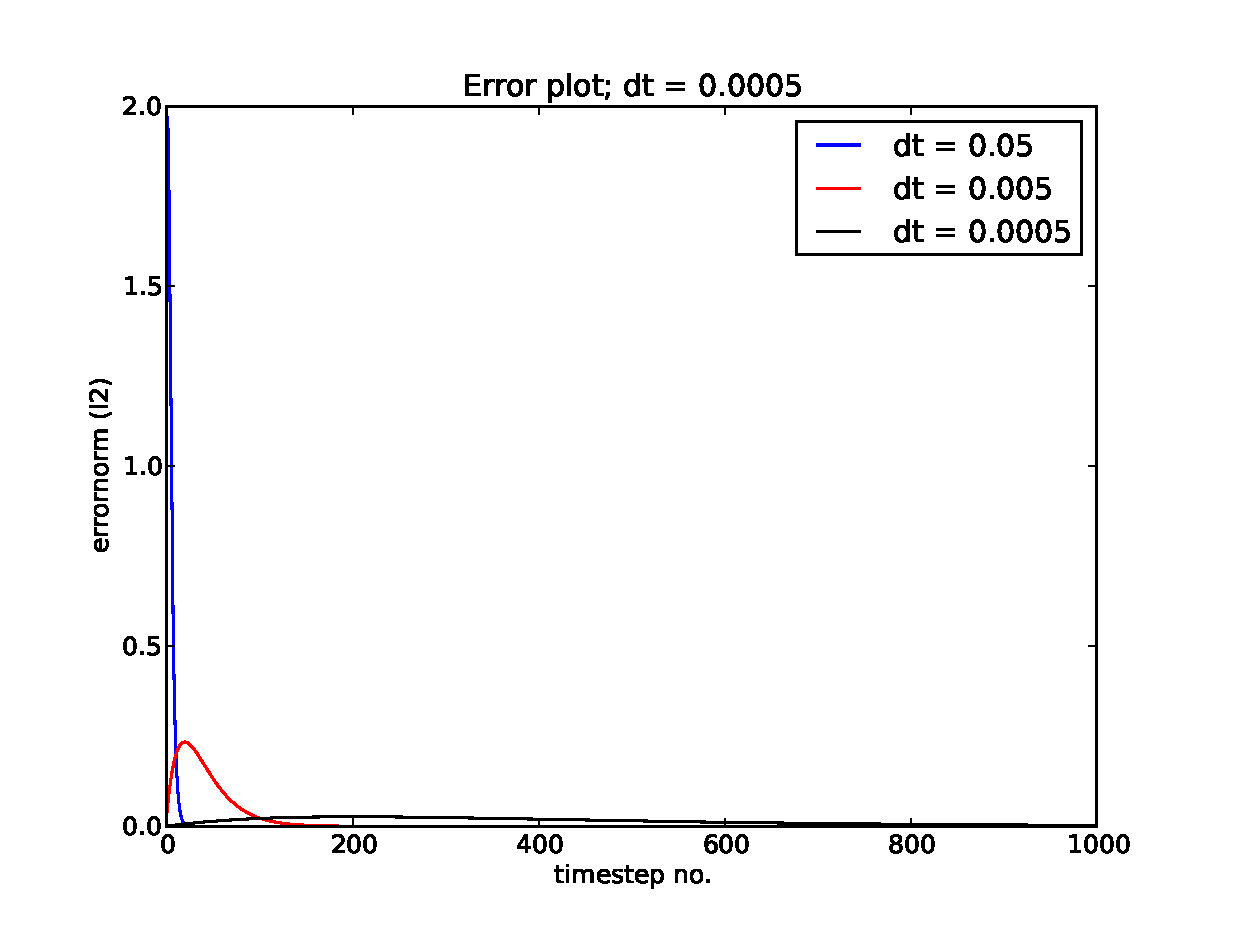
\includegraphics[width=\textwidth]{../results/experiment_18042014_1450_convergencetest_BE2D/results/errorplot.eps}
  \caption{}
 \end{subfigure}
 \caption[Error plots BE]{Error plot for the BE scheme in 1D (a) and 2D (b). Notice that the error is of the same order as the time step.}
 \label{analysis:errorplots:BE}
\end{figure}

\subsection{Verification by convergence tests}

The convergence tests are done by isolating the error term from either the time derivative or the spatial derivative, and refining the relevant discretization parameter over several simulations. 
Figures \ref{analysis:convergence_tests:FE} and \ref{analysis:convergence_tests:BE} verify that the error associated with the time derivative is of the expected order while figure \ref{analysis:spatial_convergence_tests} verifies the error from the spatial derivative for the BE scheme.

\begin{figure}[h]
% Convergence tests for FE in 1D (a) and 2D (b)
\centering
 \begin{subfigure}{0.49\textwidth}
  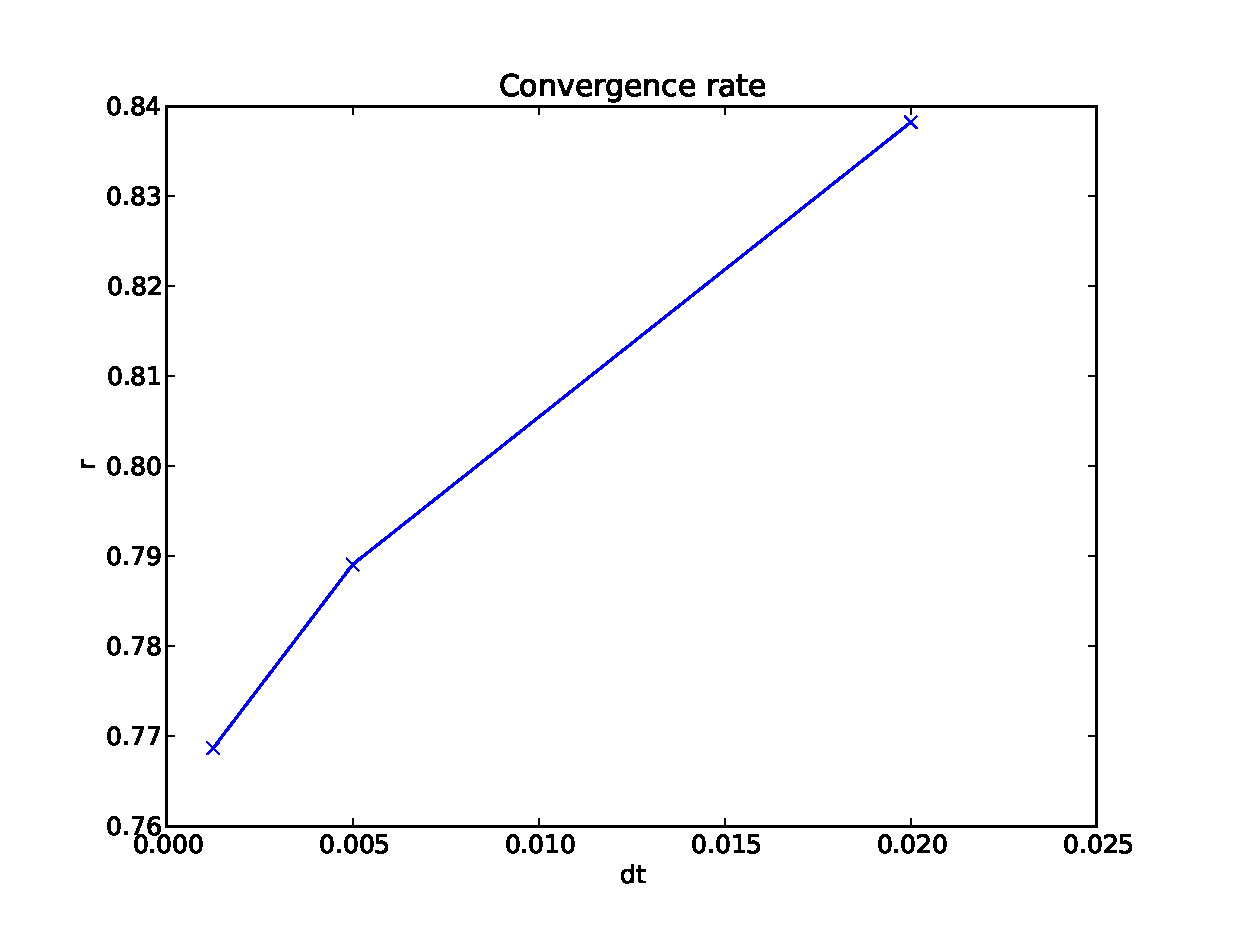
\includegraphics[width=\textwidth]{../results/experiment_18042014_1014_convergencetest_FE1D/results/ConvergenceTest.eps}
  \caption{}
 \end{subfigure}
 \begin{subfigure}{0.49\textwidth}
  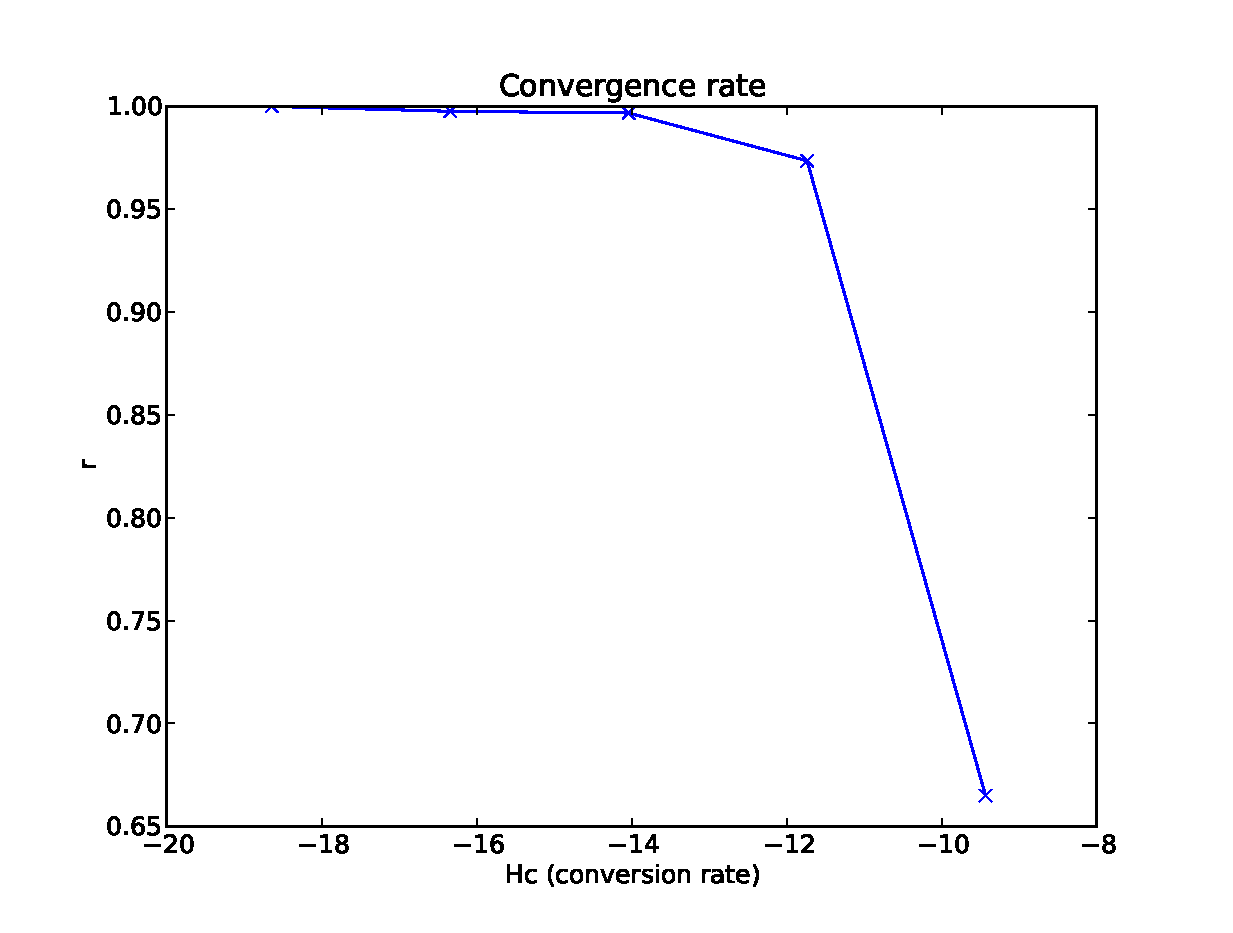
\includegraphics[width=\textwidth]{../results/experiment_29112013_1709/results/ConvergenceTest.eps}
  \caption{}
 \end{subfigure}
 \caption[Convergence tests in time FE scheme]{Convergence tests with respect to the time derivative for the FE scheme in 1D (a) and 2D (b). }
 \label{analysis:convergence_tests:FE}
\end{figure}

\begin{figure}[h]
% Convergence tests for BE in 1D (a) and 2D (b)
\centering
 \begin{subfigure}{0.49\textwidth}
  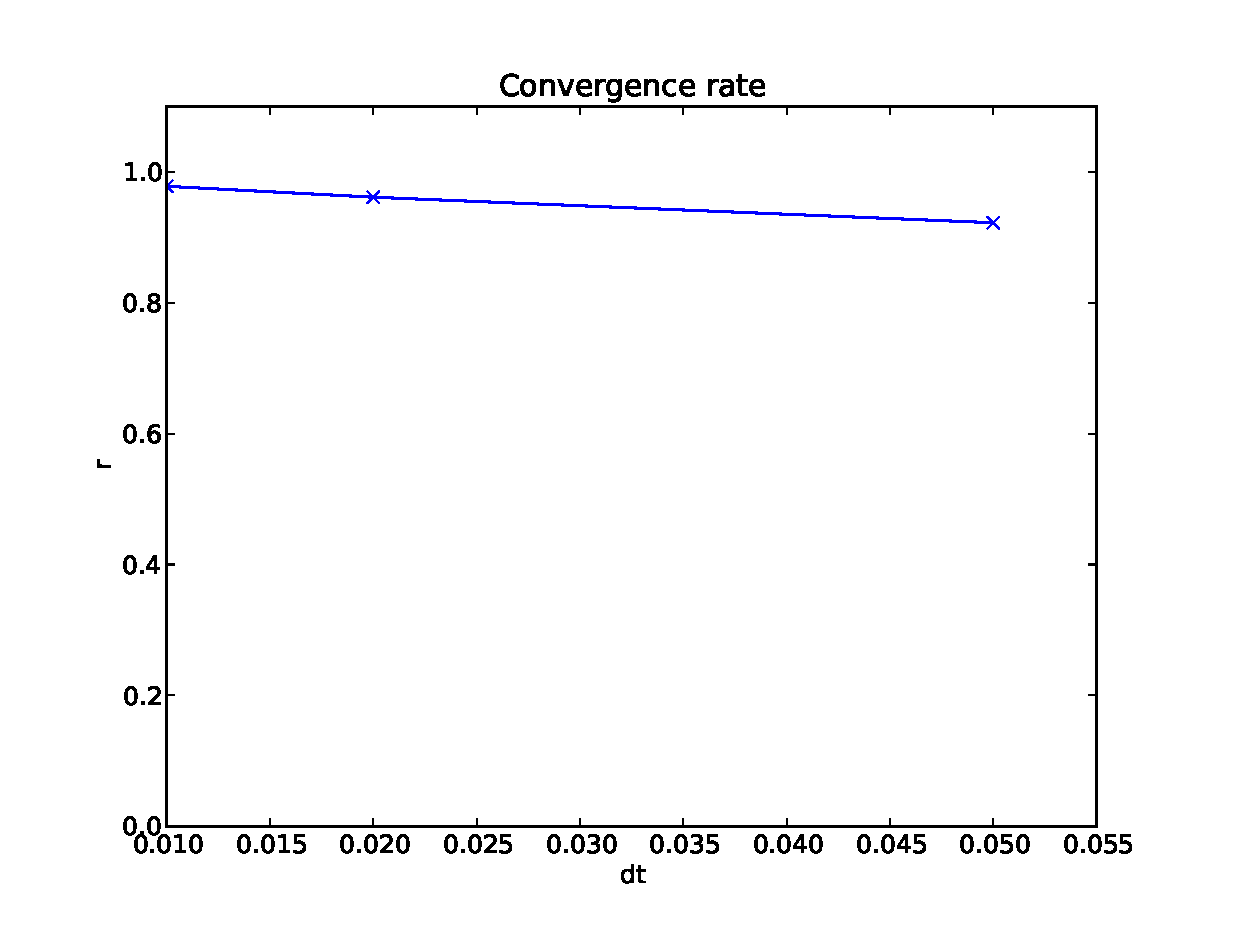
\includegraphics[width=\textwidth]{../results/experiment_14052014_0744_errorplot_BE1D/results/ConvergenceTest.eps}
  \caption{}
 \end{subfigure}
 \begin{subfigure}{0.49\textwidth}
  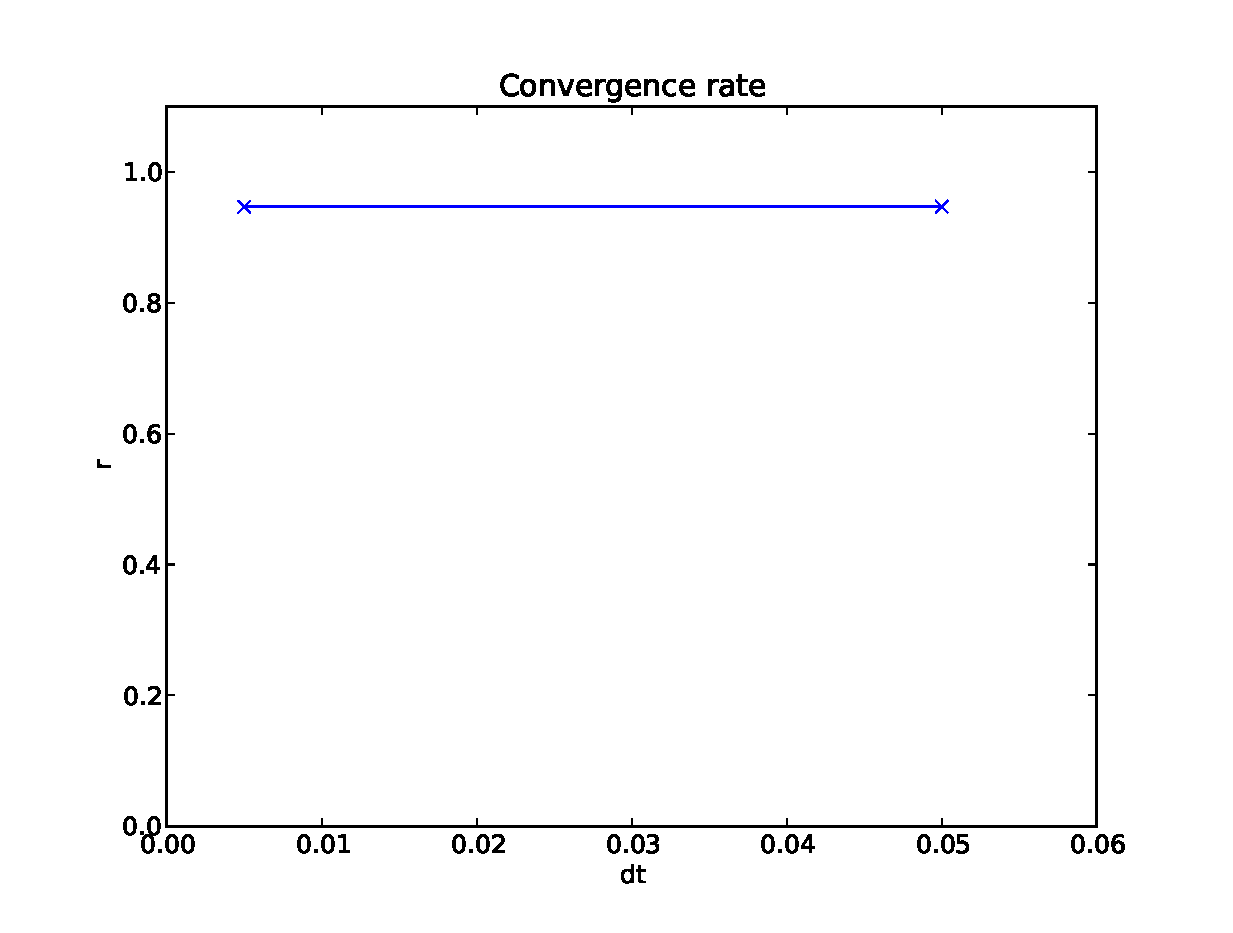
\includegraphics[width=\textwidth]{../results/experiment_18042014_1450_convergencetest_BE2D/results/ConvergenceTest.eps}
  \caption{}
 \end{subfigure}
 \caption[Convergence tests for BE scheme]{Convergence tests with respect to the time derivative for the BE scheme in 1D (a) and 2D (b).}
 \label{analysis:convergence_tests:BE}
\end{figure}

\begin{figure}[H]
% Spatial error test for the BE scheme
\centering
 \begin{subfigure}{0.49\textwidth}
  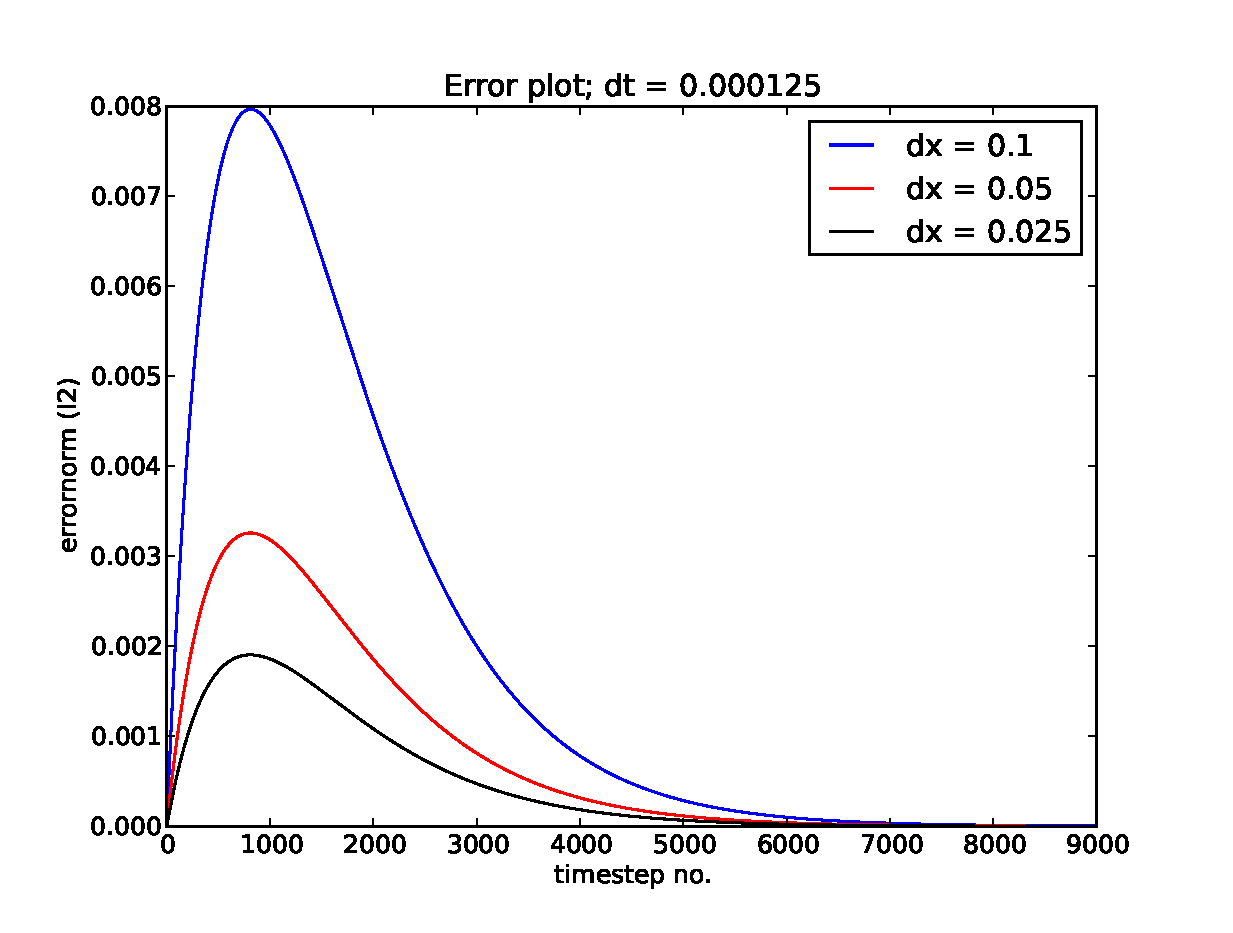
\includegraphics[width=\textwidth]{../results/experiment_14042014_1303_convergence_tests_etc/results/errorplot.eps}
  \caption{}
 \end{subfigure}
 \begin{subfigure}{0.49\textwidth}
  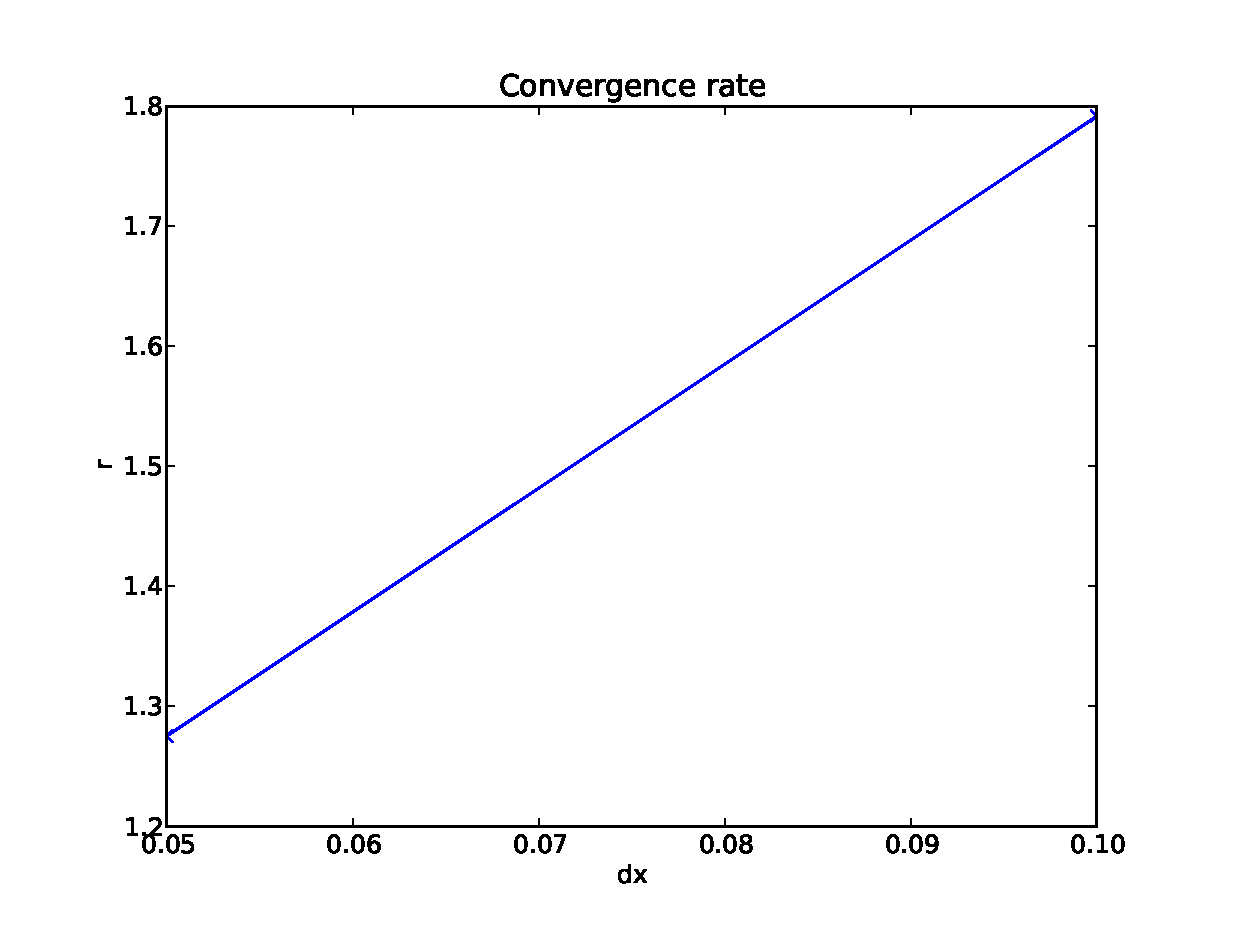
\includegraphics[width=\textwidth]{../results/experiment_14042014_1303_convergence_tests_etc/results/ConvergenceTest.eps}
  \caption{}
 \end{subfigure}
 \caption[Spatial error test for the BE scheme]{This figure shows the error from the spatial derivative (a) and the corresponding convergence test. For the smallest $\Delta x$ the spatial error is no longer completely dominant which explains the poorer convergence.}
 \label{analysis:spatial_convergence_tests}
\end{figure}
\subsection{Verification of FE scheme by exact numerical solution}

Discretization of the diffusion equation by the FE scheme yields the following numerical scheme in 1D
\begin{equation}
 u^{n+1} = D\Delta t u^n_{xx} + u^n
\end{equation}
where $u_{xx}$ denotes the double derivative of $u$ with respect to $x$. 
To illustrate how the equation is solved by the computer, the first four iterations are written out
\begin{align*}
 u^1 &= D\Delta t\, u_{xx}^0 + u^0 \\
 u^2 &= D\Delta t\, u_{xx}^1 + u^1 \\
 &= D\Delta t\left[D\Delta t u_{4x}^0 + u_{2x}^0\right] + u^0\\
 &= \left(D\Delta t\right)^2 u_{4x}^0 + 2D\Delta t u_{2x}^0+ u^0 \\
 u^3 &= D\Delta t\, u_{xx}^2 + u^2 \\
 &= D\Delta t\left[\left(D\Delta t\right)^2 u_{6x}^0 + 2D\Delta t u_{4x}^0+ u_{2x}^0\right] + \left(D\Delta t\right)^2 u_{4x}^0 + 2D\Delta t u_{2x}^0+ u^0\\
 &= \left(D\Delta t\right)^3 u_{6x}^0 + 3\left(D\Delta t\right)^2 u_{4x}^0+ 3D\Delta tu_{2x}^0 + u^0 \\
 u^4 &= D\Delta t \,u_{xx}^3 + u^3 = \dots \\
 &= \left(D\Delta t\right)^4 u_{8x}^0 + 4\left(D\Delta t\right)^3 u_{6x}^0+ 6\left(D\Delta t\right)^2 u_{4x}^0 + 4D\Delta t u_{2x}^0 + u^0 
\end{align*}

\noindent From the iterations above a pattern emerges for iteration $n+1$\\
\begin{equation}
 u^{n+1} = \sum\limits_{i=0}^n {n\choose i}\left(D\Delta t\right)^iu^0_{2ix}
\end{equation}
Where $u^0$ is the initial condition
\begin{equation}
 u^0 = \cos(\pi x)
\end{equation}
The spatial derivatives are found as
\begin{align*}
 u^0_{xx} &= \frac{1}{\Delta x^2}\left(\cos(\pi(x+\Delta x)) -2\cos(\pi x) +\cos(\pi(x-\Delta x))\right) \\
 &= \frac{2}{\Delta x^2}\left(\cos(\pi\Delta x)-1\right)\cos(\pi x)\\
 u^0_{4x} &= [u^0_{xx}]_{xx} \frac{1}{\Delta x^2}\left[\frac{u^0_{xx}}{\cos(\pi x)}\left(\cos(\pi(x+\Delta x)) -2\cos(\pi x) +\cos(\pi(x-\Delta x))\right)\right]\\
 &= \frac{4}{\Delta x^2}\left(\cos(\pi\Delta x)-1\right)^2\cos(\pi x)\\
 &\dots
\end{align*}
The pattern continues allowing the final numerical exact solution to be expressed below.
\begin{equation}\label{numerical_solution}
  u^{n+1} = \sum\limits_{i=0}^n {n\choose i}\left(D\Delta t\right)^i\frac{2^i}{\Delta x^{2i}}\left(\cos(\pi\Delta x)-1\right)^i\cos(\pi x)
\end{equation}
By construction the Neumann boundary conditions are fulfilled since $\frac{\d \cos(\pi x)}{\d x} = -\pi\sin(\pi x)$ and $\sin(0) = \sin(\pi) = 0$. \\

Although the FE scheme is expected to reproduce \eqref{numerical_solution} to machine precision ($\epsilon \approx 10^{-16}$) there are two problems with the solution which will have an effect on the error:
\begin{itemize}
 \item $\Delta x^{2i}$ will quickly tend to zero, and the computer will interpret it as zero. This will cause division by zero, which again results in ``Not a number'' (nan) and ruins the simulation. Testing if $\Delta x^{2i}>0$ and returning zero if the test fails will fix the problem. The argumentation for ignoring the troublesome terms is given below.
 \item ${n\choose i}$ goes to infinity for large $n$ and $i$. The computer can only represent numbers up to $\sim10^{308}$, which limits the number of steps to $170$ since $n!>10^{308}$ for $n>170$.
\end{itemize}

As a side note, equation \eqref{numerical_solution} illustrates how the stability criterion for the FE scheme comes into place. 
In the numerical exact solution the exponential which is found in the exact solution to the PDE (eq. \ref{manufactured_solution}) is replaced by an amplification factor $A^n$.
This amplification factor can be found in equation \eqref{numerical_solution} as 
\begin{equation}
A^n = \left(\frac{2D\Delta t}{\Delta x^2}\right)^i
\end{equation}
Inserting a time step larger than the stability criterion ($\Delta t \leq \frac{\Delta x^2}{2D}$) will make the amplification factor $A$ larger than one which in turn will make the solution blow up. \\
The stability criterion also illustrates why the terms where 
$$ \frac{1}{\Delta x^{2i}} \to \infty$$
 can be dropped. 
 By the stability criterion, the time step will cancel out $\Delta x^2$, and the result will be a number smaller than 1 raised to a rather large power, $i$, resulting in a number comparable to zero.\\
 
 The results from comparing a 1D simulation to the numerical exact is shown in Figure \ref{numerical_exact_FE:1D}. 
 As expected the error is larger than machine precision by at most two orders of magnitude because of accumulating error terms from the dropped terms in eq. \eqref{numerical_solution}.
 
 Using the same method as in the 1D case, a numerical exact solution can be found to the 2D FE scheme. 
 \begin{equation}\label{exact_numerical_solution_2d}
 u^{n+1} = \sum\limits^n_{i=0}{n\choose i}\left(D\Delta t\right)^i\left[2^{i-1}\cos(\pi x)\cos(\pi y)\left(\frac{(\cos(\pi\Delta x))^i}{\Delta x^{2i}} +\frac{(\cos(\pi\Delta y))^i}{\Delta y^{2i}}\right)\right]
\end{equation}

The same problems as in the 1D case will apply to equation \eqref{exact_numerical_solution_2d} with the same solutions. 
Figure \ref{numerical_exact_FE:2D} shows how the 2D simulation compares to the numerical exact solution. 
As was the case in 1D the error is larger than machine precision, but much smaller than $\Delta t$.
% suggesting that the scheme is implemented correctly.

\begin{figure}[H]
 \centering
 \begin{subfigure}{0.49\textwidth}
 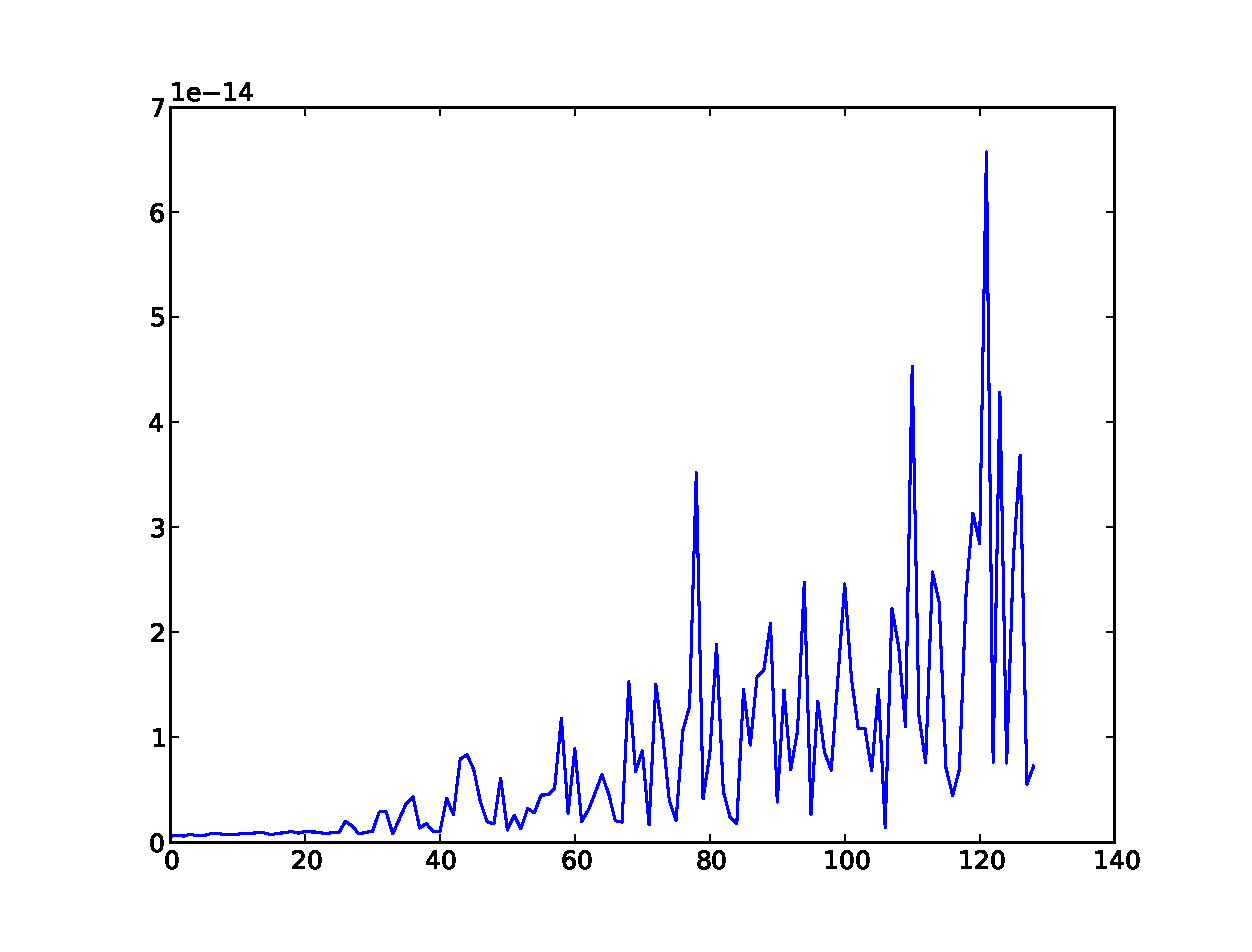
\includegraphics[width=\textwidth]{Figures/exact_numerical_1d_n130.eps}
  \caption{}
  \label{numerical_exact_FE:1D}
 \end{subfigure}
 \begin{subfigure}{0.49\textwidth}
 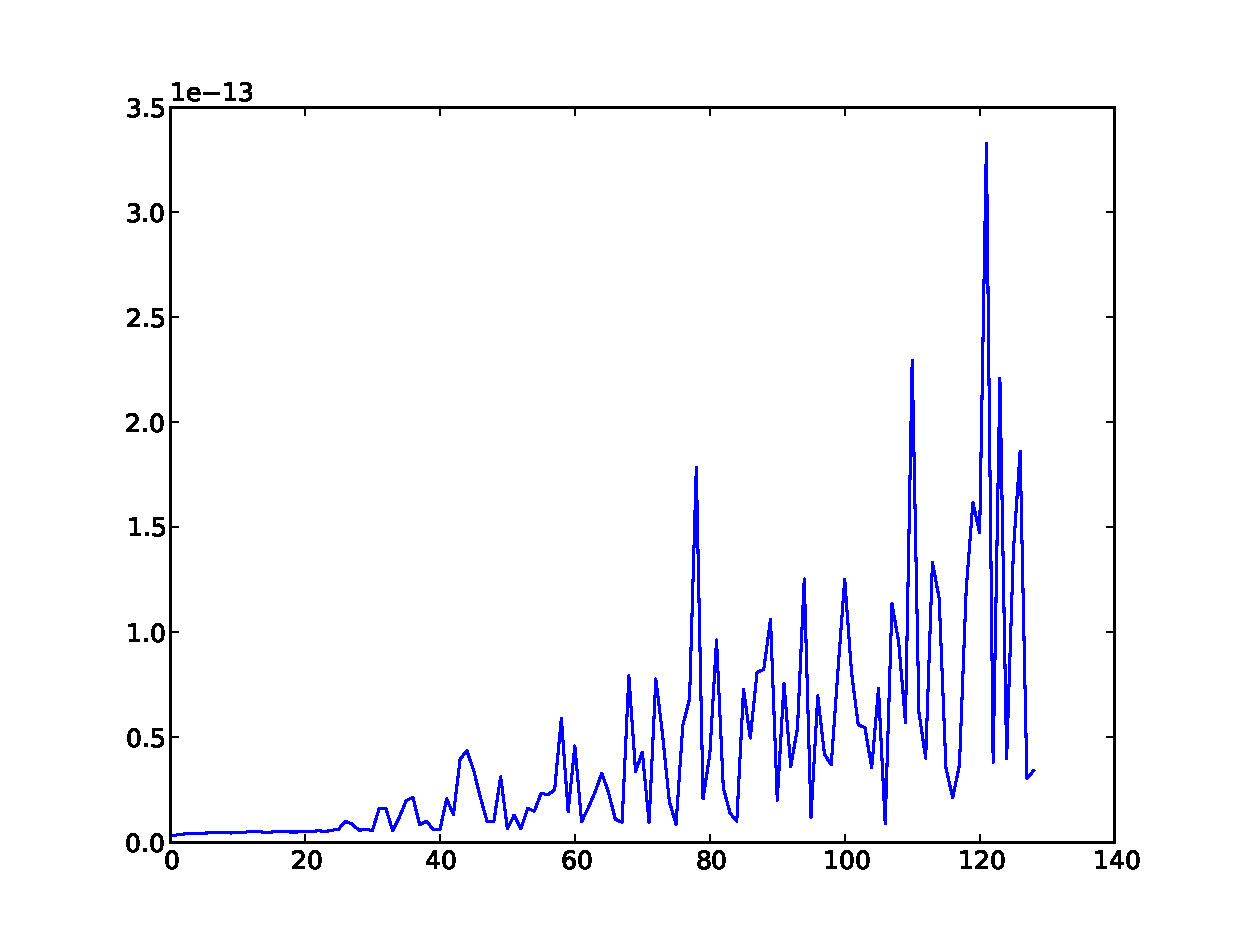
\includegraphics[width=\textwidth]{Figures/exact_numerical_2d_n130.eps}
  \caption{}
  \label{numerical_exact_FE:2D}
 \end{subfigure}
 \caption[Numerical exact error plots FE]{Numerical solution from the FE scheme in 1D (a) and 2D (b) versus the exact numerical solution of the FE scheme.
 Some of the terms in the numerical exact solutions are ignored to prevent overflow and this is responsible for the increasing error which is slightly larger than machine precision.}
 \label{numerical_exact_FE}
\end{figure}


\subsection{Verification of BE scheme by exact numerical solution}

The exact numerical solution to the BE scheme is found by solving the linear system which arises from the discretization. 
Given the $n$'th time step, the next time step is found by

\begin{align*}
 \mathbf M \mathbf u^{n+1} &= \mathbf{u}^n \\
 \mathbf{u}^{n+1} &= \mathbf{M}^{-1} \mathbf{u}^n \\
 &= \mathbf{M}^{-1}\left(\mathbf{M}^{-1} \mathbf{u}^{n-1}\right)
\end{align*}

\noindent Doing the separation to the end relates the $n$'th time step to the initial condition
\begin{equation}\label{BE_numex}
 \vec u^{n+1} = \left(\mathbf M^{-1}\right)^{n+1} \vec u^0
\end{equation}

\noindent Where $\left(\mathbf M^{-1}\right)^{n+1}$ is the inverse of $\mathbf M$ to the $n+1$'th power.\\

Taking the inverse of $\mathbf M$ will result in a dense matrix where a lot of the entries are close to zero (e.g. $10^{-20}$). 
Doing calculations with such a matrix gives a lot of round off errors which will reduce the accuracy of the numerical exact. 
The error should theoretically be machine precision, but is expected to at least be much smaller than $\Delta t$. 
Errors from both 1D and 2D simulations are shown in Figure \ref{numex:BE_errorplot}

\begin{figure}[H]
 \centering
 \begin{subfigure}{0.49\textwidth}
 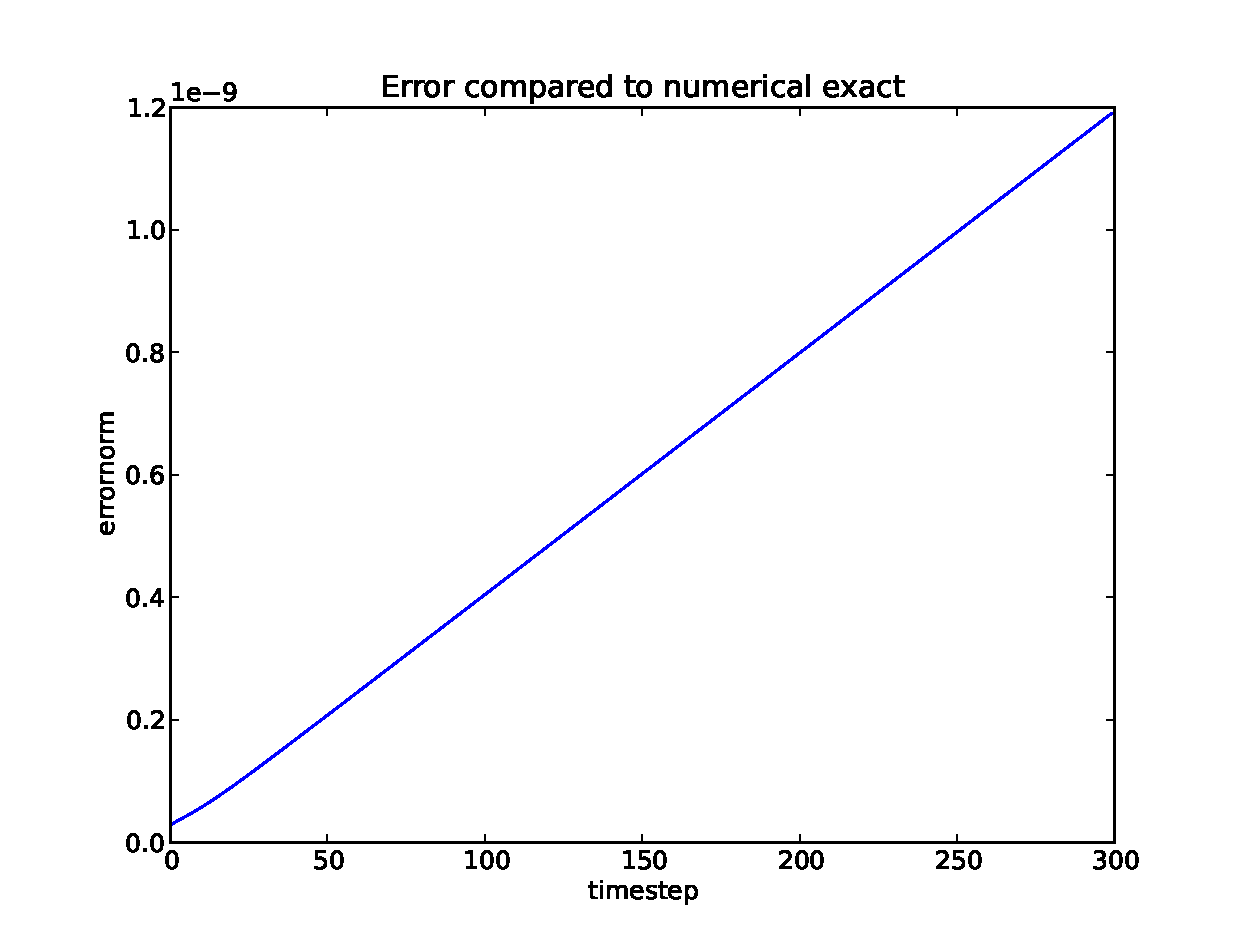
\includegraphics[width=\textwidth]{../results/experiment_14042014_0759_BE1D_numerical_exact/results/numerical_exact.eps}
 \caption{}
\end{subfigure}
\begin{subfigure}{0.49\textwidth}
 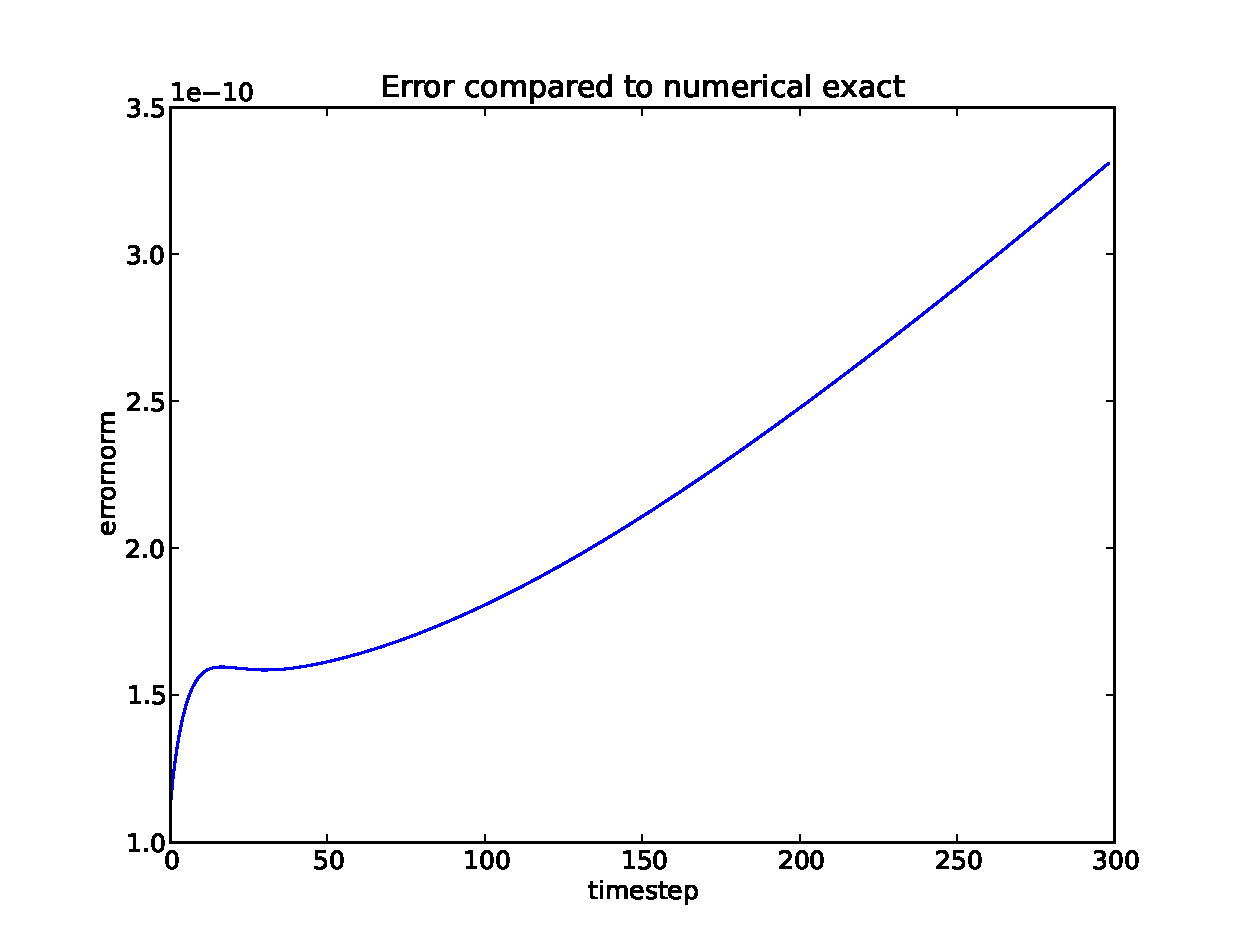
\includegraphics[width=\textwidth]{../results/experiment_30042014_0914_BE2D_numex/results/numerical_exact.eps}
 \caption{}
\end{subfigure}
 \caption[Numerical exact errorplots for BE scheme]{Plots showing the error for the BE scheme in 1D (a) and 2D (b) compared to the numerical exact solution. 
 The error is not machine precision, but significantly smaller than $\Delta t$ which for these simulations is $\Delta t=0.01$. 
 This increased error originates in the many roundoff errors in the inverted matrix where a lot of terms $10^{-16}$ and smaller.}
 \label{numex:BE_errorplot}
\end{figure}

\section{Verification of the RW solver}

The aim of this section is to verify that the implemented RW model will solve the diffusion equation with on the correct time scale, and to verify that the error term from the RW solver is dependent on the conversion factor, $Hc$. 
In order to carry out the tests a new initial condition that can easily be recreated by random walkers will be introduced.
\begin{equation}
 u(t=0,x) = H\left(x-\frac{1}{2}\right)
\end{equation}
\noindent Where $H(x)$ denotes the Heaviside step function which is defined by its properties
\begin{equation}\label{Heaviside_def}
 H(x-a) = \begin{cases}
           1\;\;x > a\\
           \frac{1}{2}\;\; x = a\\ 
           0\;\;x < a
          \end{cases}
\end{equation}
\noindent The new initial condition gives a new exact solution which is found by separation of variables as 
\begin{equation}
 u(x,t) = \frac{1}{2} + \sum\limits_{n=1}^\infty \frac{2\sin(\frac{n\pi}{2})}{n\pi}e^{-(n\pi)^2t}\cos(n\pi x)
\end{equation}

\noindent Figure \ref{ConvergenceTestRW:Hc} verifies that the error term improves by adding more walkers. And figure \ref{ConvergenceTestRW:dt} shows that the RW model will fulfill the chosen time step on the PDE level. 
The convergence is not very good, but this is expected because of the fluctuations which causes the error to fluctuate around a certain value rather than converge to zero.

\begin{figure}[h]
 \centering
\begin{subfigure}[t]{0.49\textwidth}
 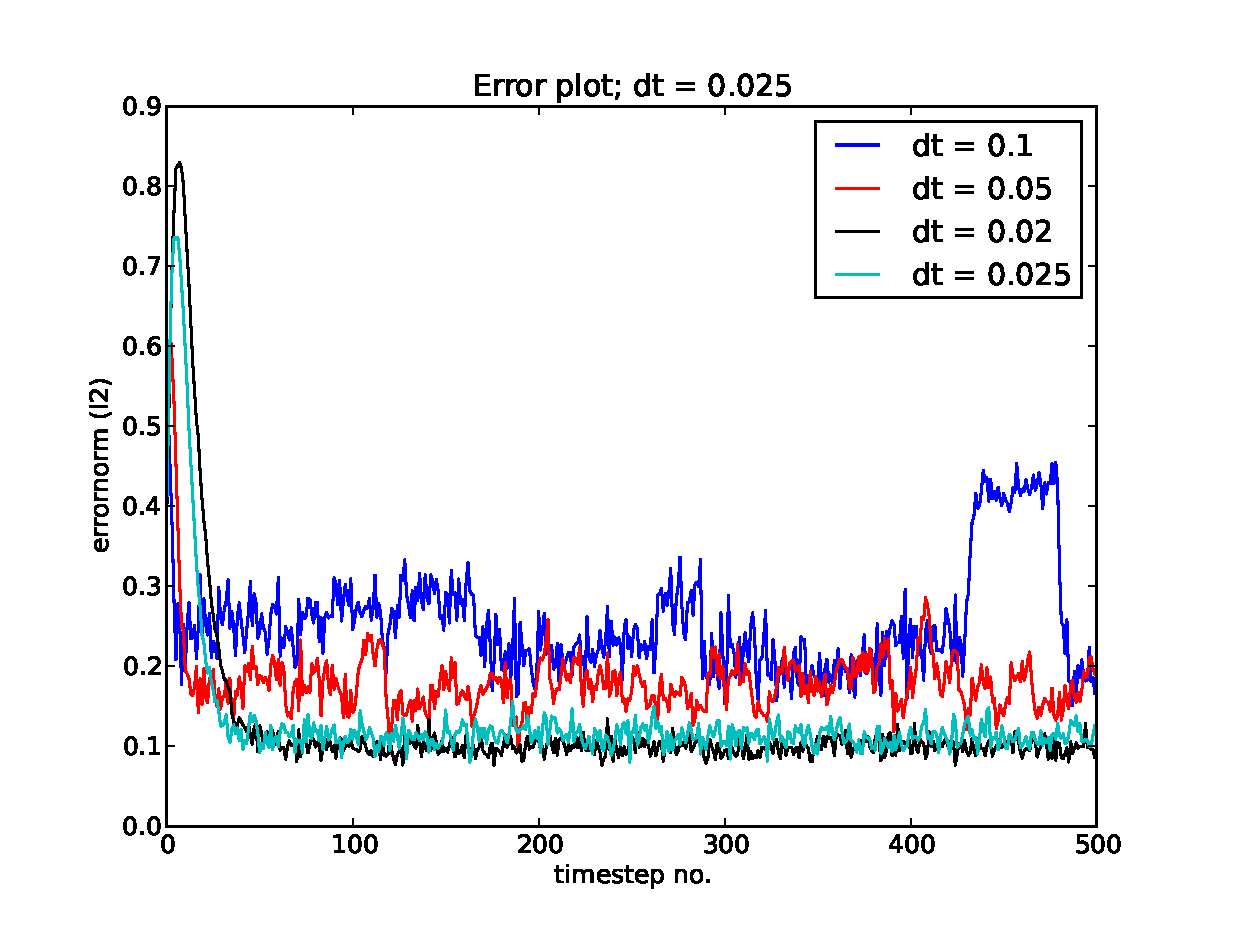
\includegraphics[width=\textwidth]{../results/experiment_01052014_1615_Redoing_RW_tests/results/errorplot.eps}
 \caption{}
 \label{ConvergenceTestRW:dt:errorplot}
\end{subfigure}
 \begin{subfigure}[t]{0.49\textwidth}
 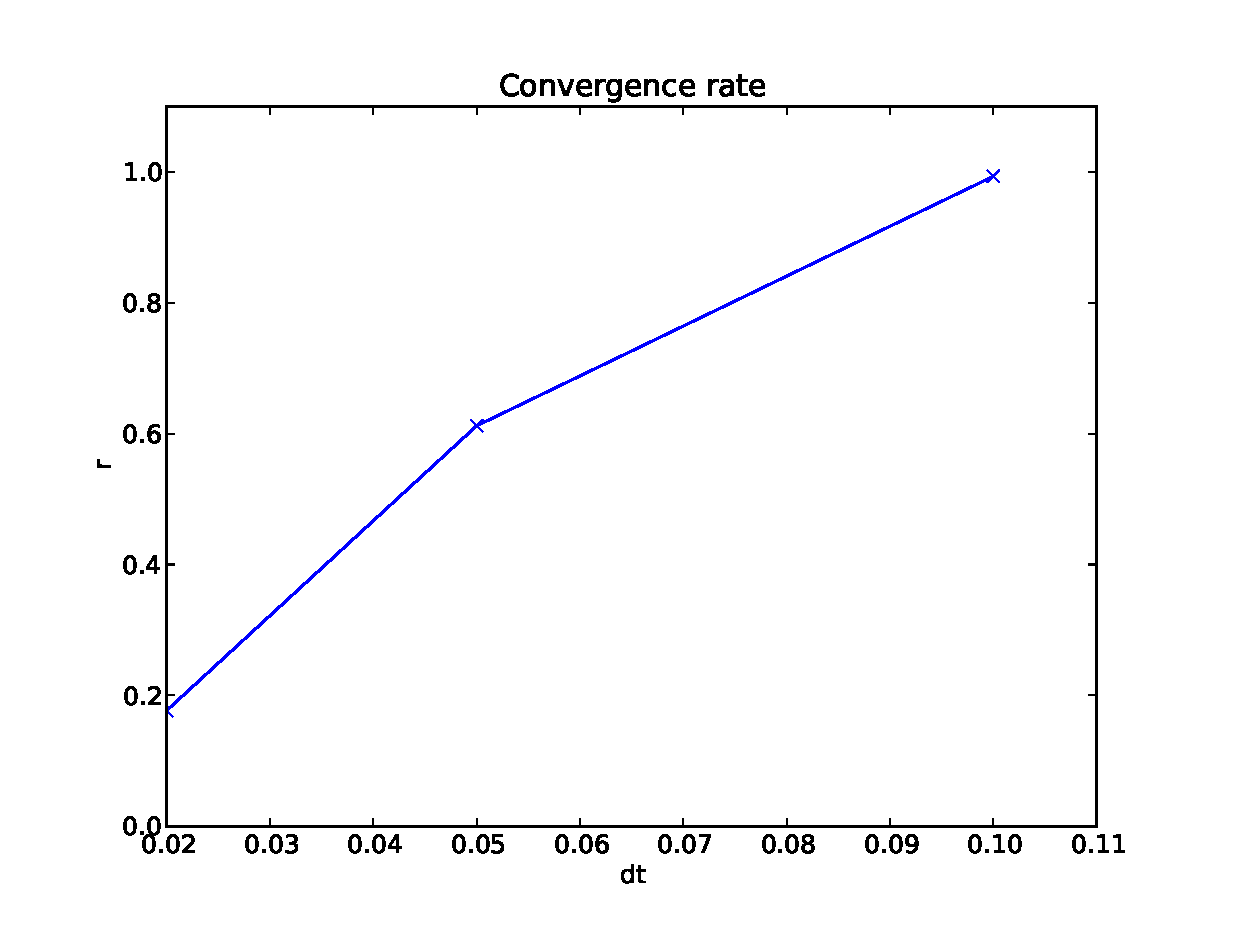
\includegraphics[width=\textwidth]{../results/experiment_01052014_1615_Redoing_RW_tests/results/ConvergenceTest.eps}
  \caption{}
 \label{ConvergenceTestRW:dt:convergence}
\end{subfigure}
\caption[]{Error plot (a) and convergence test (b) for 1D RW solver using a Heaviside step function as initial condition. In these tests both the time step and the conversion factor are changed for each simulation, and the conversion factor follows the previously proposed limit $Hc\geq\frac{1}{\Delta t^2}$. For each $\Delta t$ the RW simulation does 250 steps with a step length calculated from \eqref{theory:step_length}. The expected convergence rate is $0.5$, and to some extent this is achieved here, note however that due to fluctuations in the solution getting a good error measure is difficult and beyond our control.}
 \label{ConvergenceTestRW:dt}
\end{figure}
\begin{figure}[h]
 \centering
 \begin{subfigure}[t]{0.48\textwidth}
  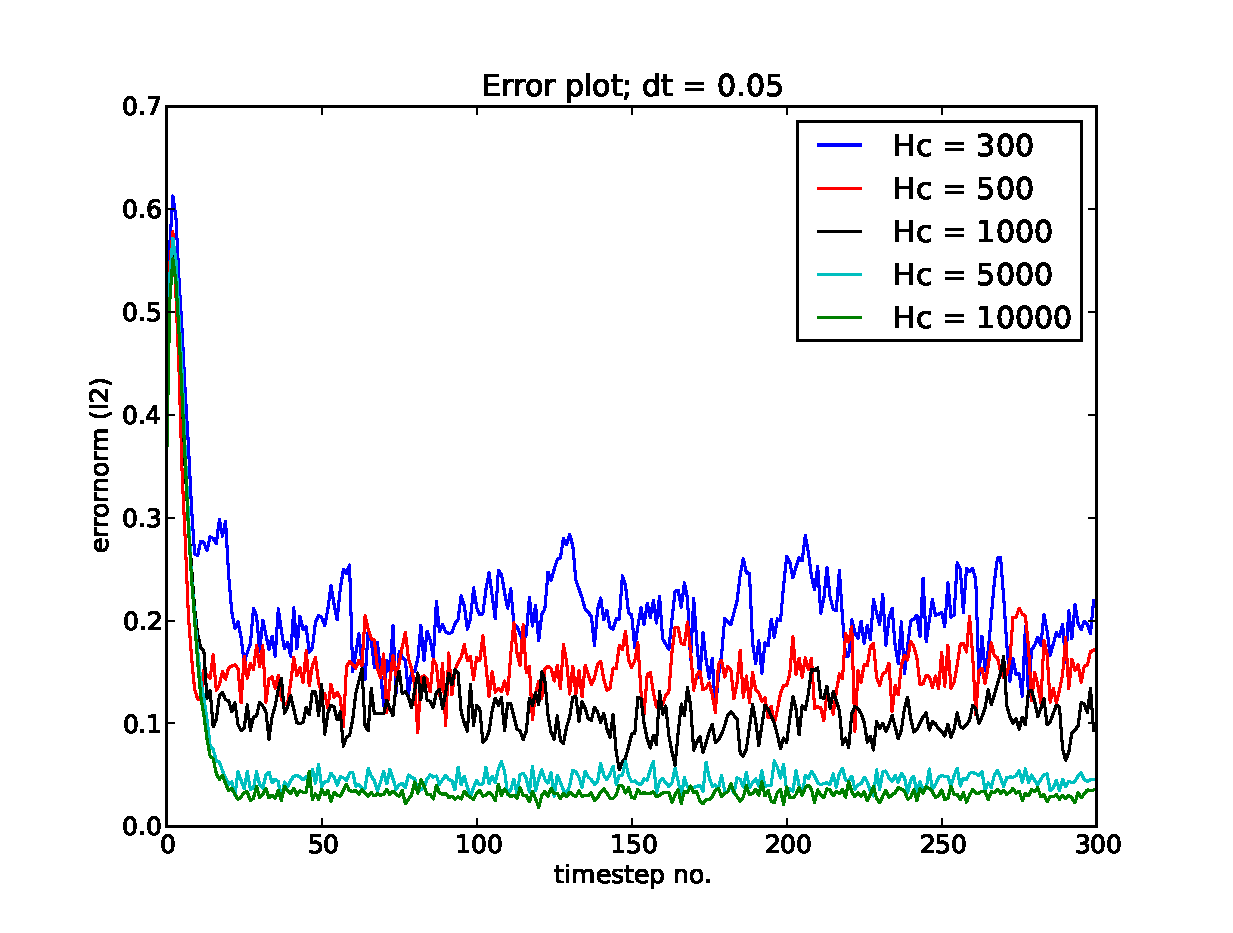
\includegraphics[width=\textwidth]{../results/experiment_02052014_0747_Redoing_RW_tests_Hc/results/errorplot.eps}
 \end{subfigure}
\begin{subfigure}[t]{0.48\textwidth}
 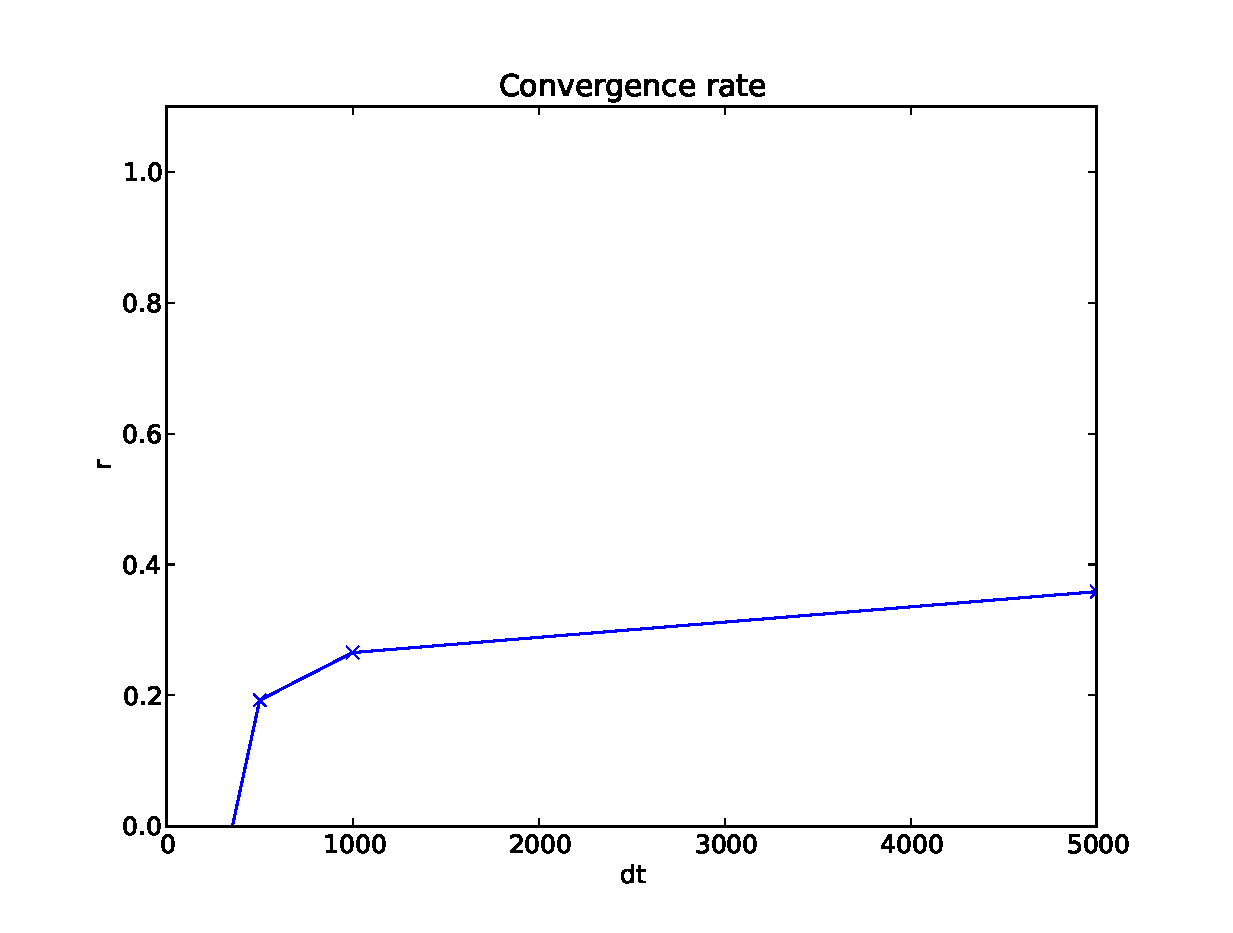
\includegraphics[width=\textwidth]{../results/experiment_02052014_0747_Redoing_RW_tests_Hc/results/ConvergenceTest.eps}
\end{subfigure}
\caption[Test RW]{As a comparison to Figures \ref{ConvergenceTestRW:dt} this test has been done for the same 1D Heaviside step function as initial condition, but keeps the time step fixed at $\Delta t = 0.05$ and increases the conversion factor. The convergence rate (fig. b) is worse than for the time convergence test, and seems to reach a limit where increasing the number of walkers has little effect on the error.}
\label{ConvergenceTestRW:Hc}
\end{figure}
\clearpage
\section{Verification of the hybrid solver}

This section aims to achieve first order convergence in time for the hybrid solver by introducing a sufficient number of walkers. 
Effects of varying the number of mesh points affected by the RW solver will also be illustrated. \\

The number of walkers needed to achieve first order convergence in time for the hybrid solver is governed by 
\begin{equation}
 Hc\geq\frac{1}{\Delta t^2}
\end{equation}
\noindent This demand makes use of the FE scheme difficult because of the stability criterion, and so all tests are done with the BE scheme. 
Figure \ref{combined_BE1d} shows first order convergence for the hybrid model.

\begin{figure}[H]
 \centering
 \begin{subfigure}[b]{0.48\textwidth}
 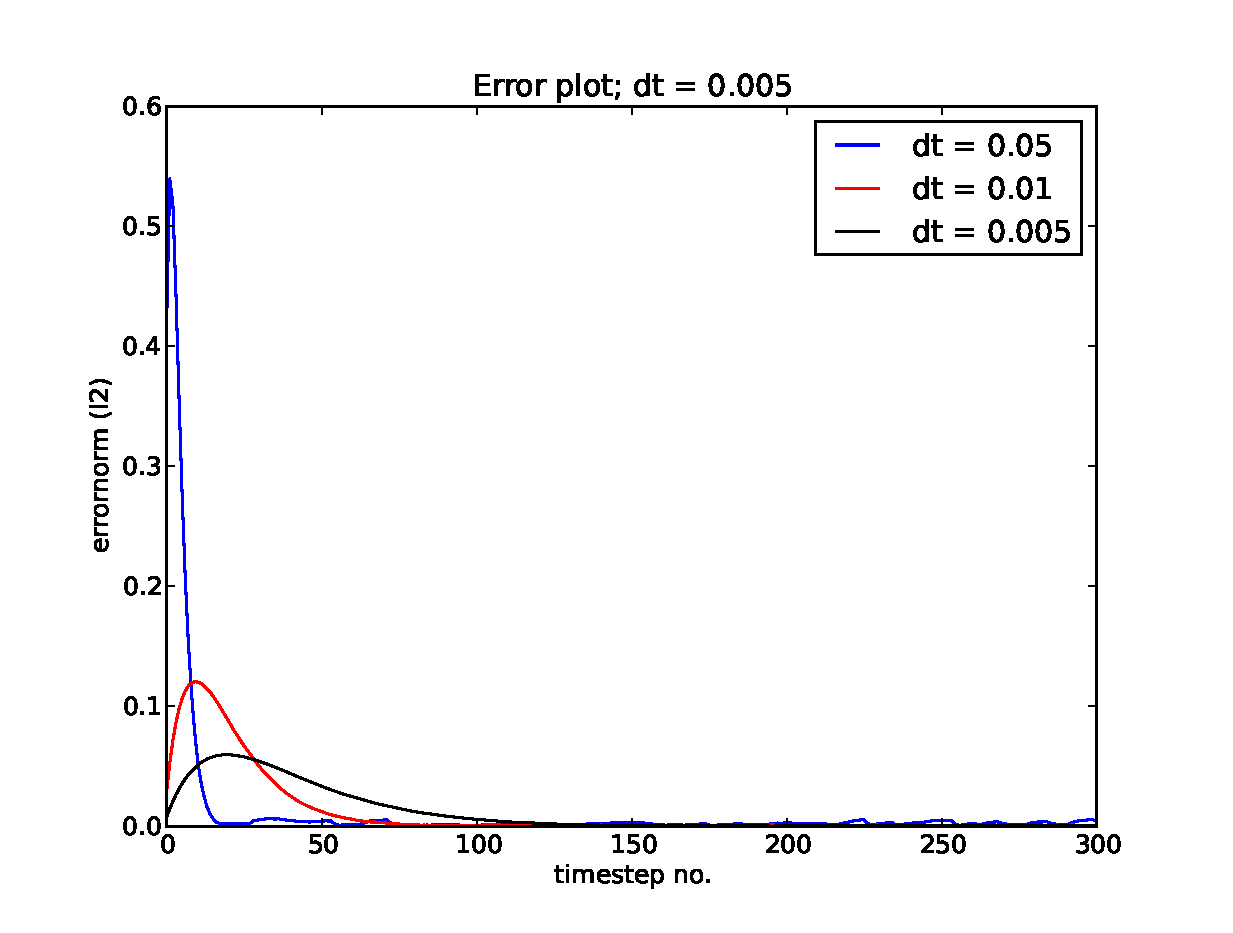
\includegraphics[width=\textwidth]{../results/experiment_15042014_0608_convergence_tests_etc/results/errorplot.eps}
\caption{}  
 \label{combined_BE1d:errorplot}
 \end{subfigure}
 \begin{subfigure}[b]{0.48\textwidth}
  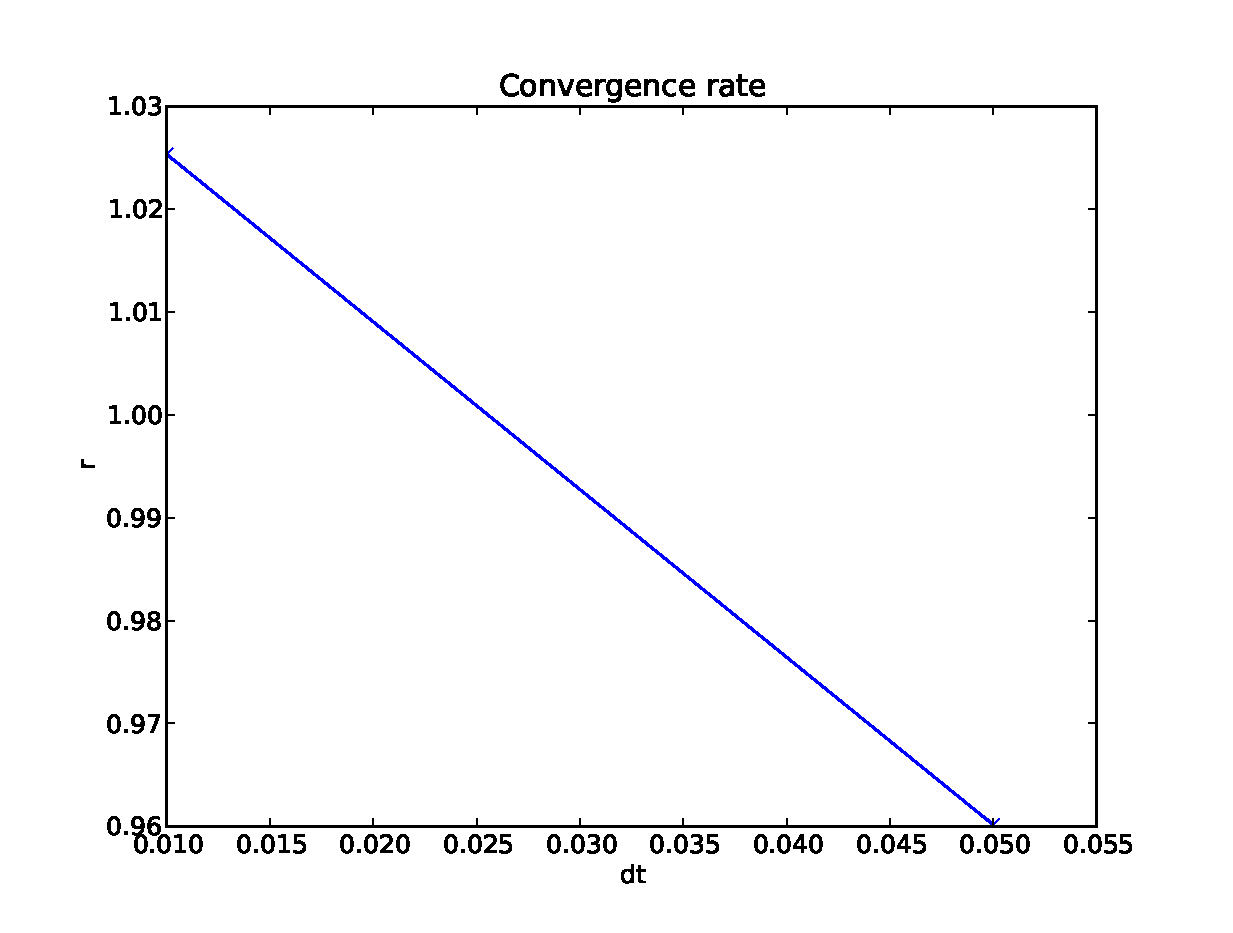
\includegraphics[width=\textwidth]{../results/experiment_15042014_0608_convergence_tests_etc/results/ConvergenceTest.eps}
  \caption{}
   \label{combined_BE1d:convergence}
 \end{subfigure}
 \caption[Error test for BE combined with RW in 1D]{\ref{combined_BE1d:errorplot} shows the error plot for a test where $\Delta x$ was fixed at $\Delta x = \frac{1}{100}$ and $\Delta t$ was reduced from $0.05$ to $0.01$ and finally to $0.005$. 
 The conversion rate, $Hc$ was updated for each simulation to have the value $Hc = \frac{1}{\Delta t^2}$, meaning the error from the walkers should be smaller than the error from the time derivative. 
 Walkers are placed on 10\% of the mesh from $x=0.4$ to $x=0.5$. 
 \ref{combined_BE1d:convergence} shows the convergence rate in time for the same test.}
 \label{combined_BE1d}
\end{figure}

Decreasing or increasing the relative size of the microscopic model as serious effects on the error and is illustrated in figure \ref{testing_walk_area_size_BE}

\begin{figure}[H]
\centering
\begin{subfigure}[b]{0.48\textwidth}
 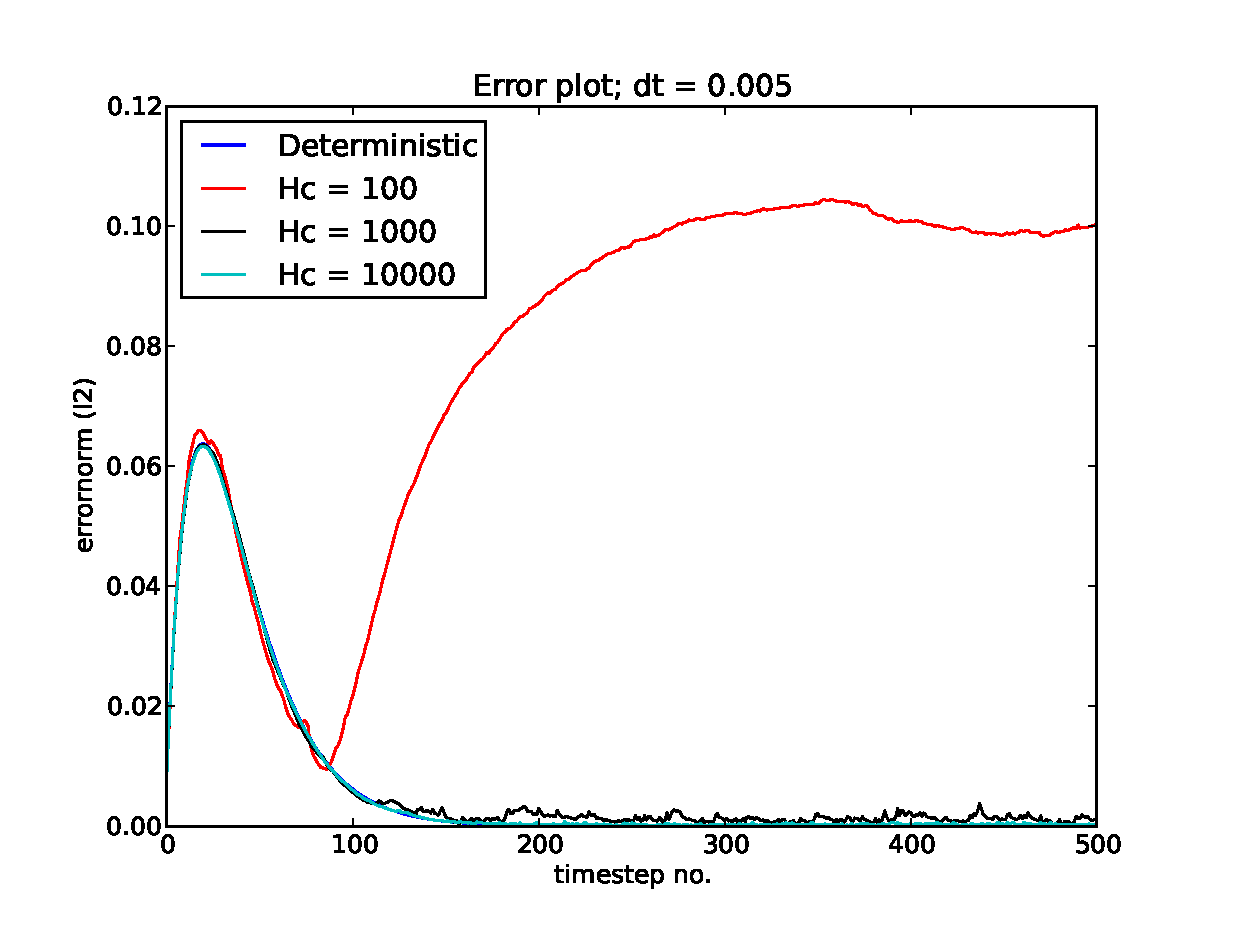
\includegraphics[width=\textwidth]{../results/experiment_16042014_1139_convergence_tests_etc/results/errorplot.eps}
 \caption{Having walkers on 5\% of the mesh points.}
 \label{errorplot_BE1D_walk_5_percent}
\end{subfigure}
\begin{subfigure}[b]{0.48\textwidth}
 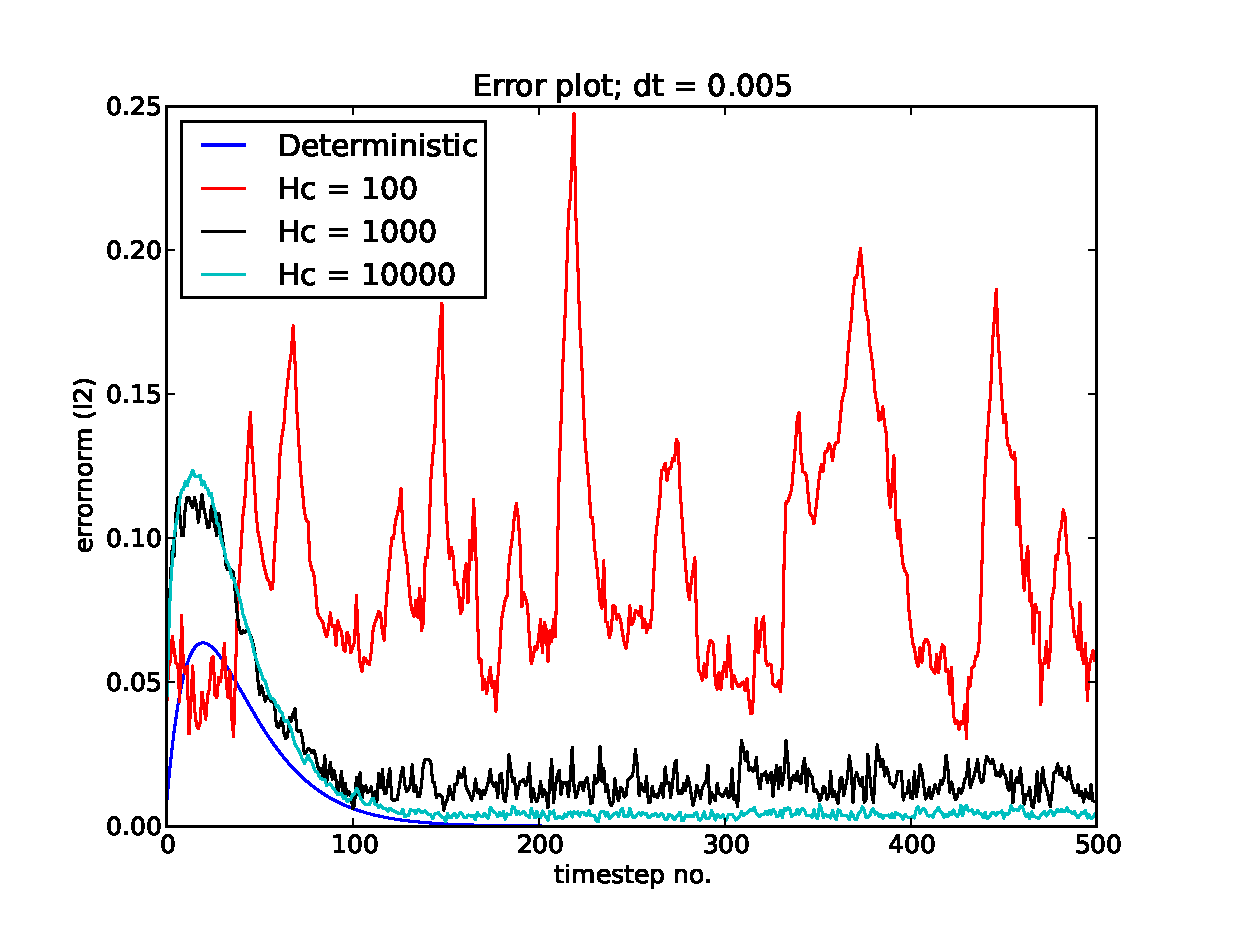
\includegraphics[width=\textwidth]{../results/experiment_16042014_1202_tests_35percent_walkers/results/errorplot.eps}
 \caption{Having walkers on 35\% of the mesh points.}
 \label{errorplot_BE1D_walk_35_percent}
\end{subfigure}
\caption[Effects of increasing relative size of walk area]{The effect of increasing the size of the walk area for a fixed $\Delta t = 0.05$ and $\Delta x = 0.01$ using the BE discretization.}
\label{testing_walk_area_size_BE}
\end{figure}